\chapter{Experimenteel Onderzoek}
\label{ch:experiment}

In het voorgaande hoofdstuk werd de ontwikkeling van de proof-of-concept softwareapplicatie uitvoerig besproken.
Voor ontwikkelingsdoeleinden werd gebruik gemaakt van een dataset die thuis werd opgenomen met de Tobii Pro Glasses 3.
Deze dataset was echter niet geschikt voor evaluatie van de uiteindelijke analysemethoden, aangezien ze door de onderzoeker zelf werden opgenomen en geen objecten bevatten die relevant zijn voor de zorgcontext.
Om een dataset te verkrijgen die wel aan deze kwaliteitseisen voldoet, werd er een experiment opgezet in het Zorglab van HoGent waarin studenten gevraagd om de eyetracker te dragen en te kijken naar verschillende objecten.
De opzet, uitvoering en de resulterende data van dit experiment worden in dit hoofdstuk nader toegelicht.

\section{Doelstellingen van het Experiment}

Het hoofddoel van het experiment was om een dataset te creëren die als grondwaarheid kon dienen voor het valideren van de twee kernmetrieken van de PoC applicatie:
\begin{itemize}
    \item De objecten die de studenten hebben bekeken.
    \item De tijdsduur dat de studenten naar deze objecten hebben gekeken.
\end{itemize}
Om deze validatie mogelijk te maken, werden twee soorten opnames gegenereerd. 
Ten eerste werden er zogenaamde \textit{kalibratieopnames} gemaakt door de onderzoeker zelf. 
Deze dienden primair om de computervisiemodellen binnen de analyses te initialiseren met de visuele kenmerken van de te detecteren objecten. 
Ten tweede werden er \textit{evaluatieopnames} verzameld waarbij studenten de eyetracker droegen en de observatietaak uitvoerden. 
Deze laatste categorie vormt de kern van de te analyseren data waarvoor de ground-truth werd vastgesteld.

Naast het genereren van deze ground-truth, had het experiment ook als doel om de robuustheid van de ontwikkelde analysemethoden te onderzoeken. 
Dit omvatte het evalueren van de prestaties van het systeem onder invloed van verschillende factoren, waaronder:
\begin{itemize}
    \item De invloed van \textbf{variërende kijkafstanden tot objecten} op de detectieaccuraatheid, resulterend in variaties in objectgrootte en detail in het camerabeeld.
    \item De prestaties van de modellen bij \textbf{diverse objectkarakteristieken}, zoals verschillen in vorm, grootte, textuur en mate van transparantie.
    \item De impact van \textbf{wisselende achtergronden} op de betrouwbaarheid van de objectherkenning.
\end{itemize}

\section{Opzet van het Experiment}

De concrete uitwerking van het experiment omvatte de inrichting van de experimentele omgeving, de keuze van kritische objecten, het opstellen van een gestandaardiseerde procedure, en de selectie van deelnemers.

\subsection{Experimentele Omgeving en Materialen}

De experimentele opnames vonden plaats in het Zorglab van HOGENT, dat beschikt over verschillende gesimuleerde zorgomgevingen. 
Voor deze bachelorproef werd specifiek gebruik gemaakt van de ruimte die is ingericht als een \textbf{woonkameromgeving}. 
Deze setting omvat typische elementen zoals een zithoek met een zetel, een keukengedeelte en een eettafel. 
Hoewel het Zorglab ook een gesimuleerde ziekenhuiskamer met twee bedden ter beschikking stelt, werd omwille van praktische overwegingen, 
zoals de positionering van objecten en de bewegingsvrijheid voor de deelnemers, gekozen voor de woonkameropstelling.

\begin{figure}[H]
  \centering
  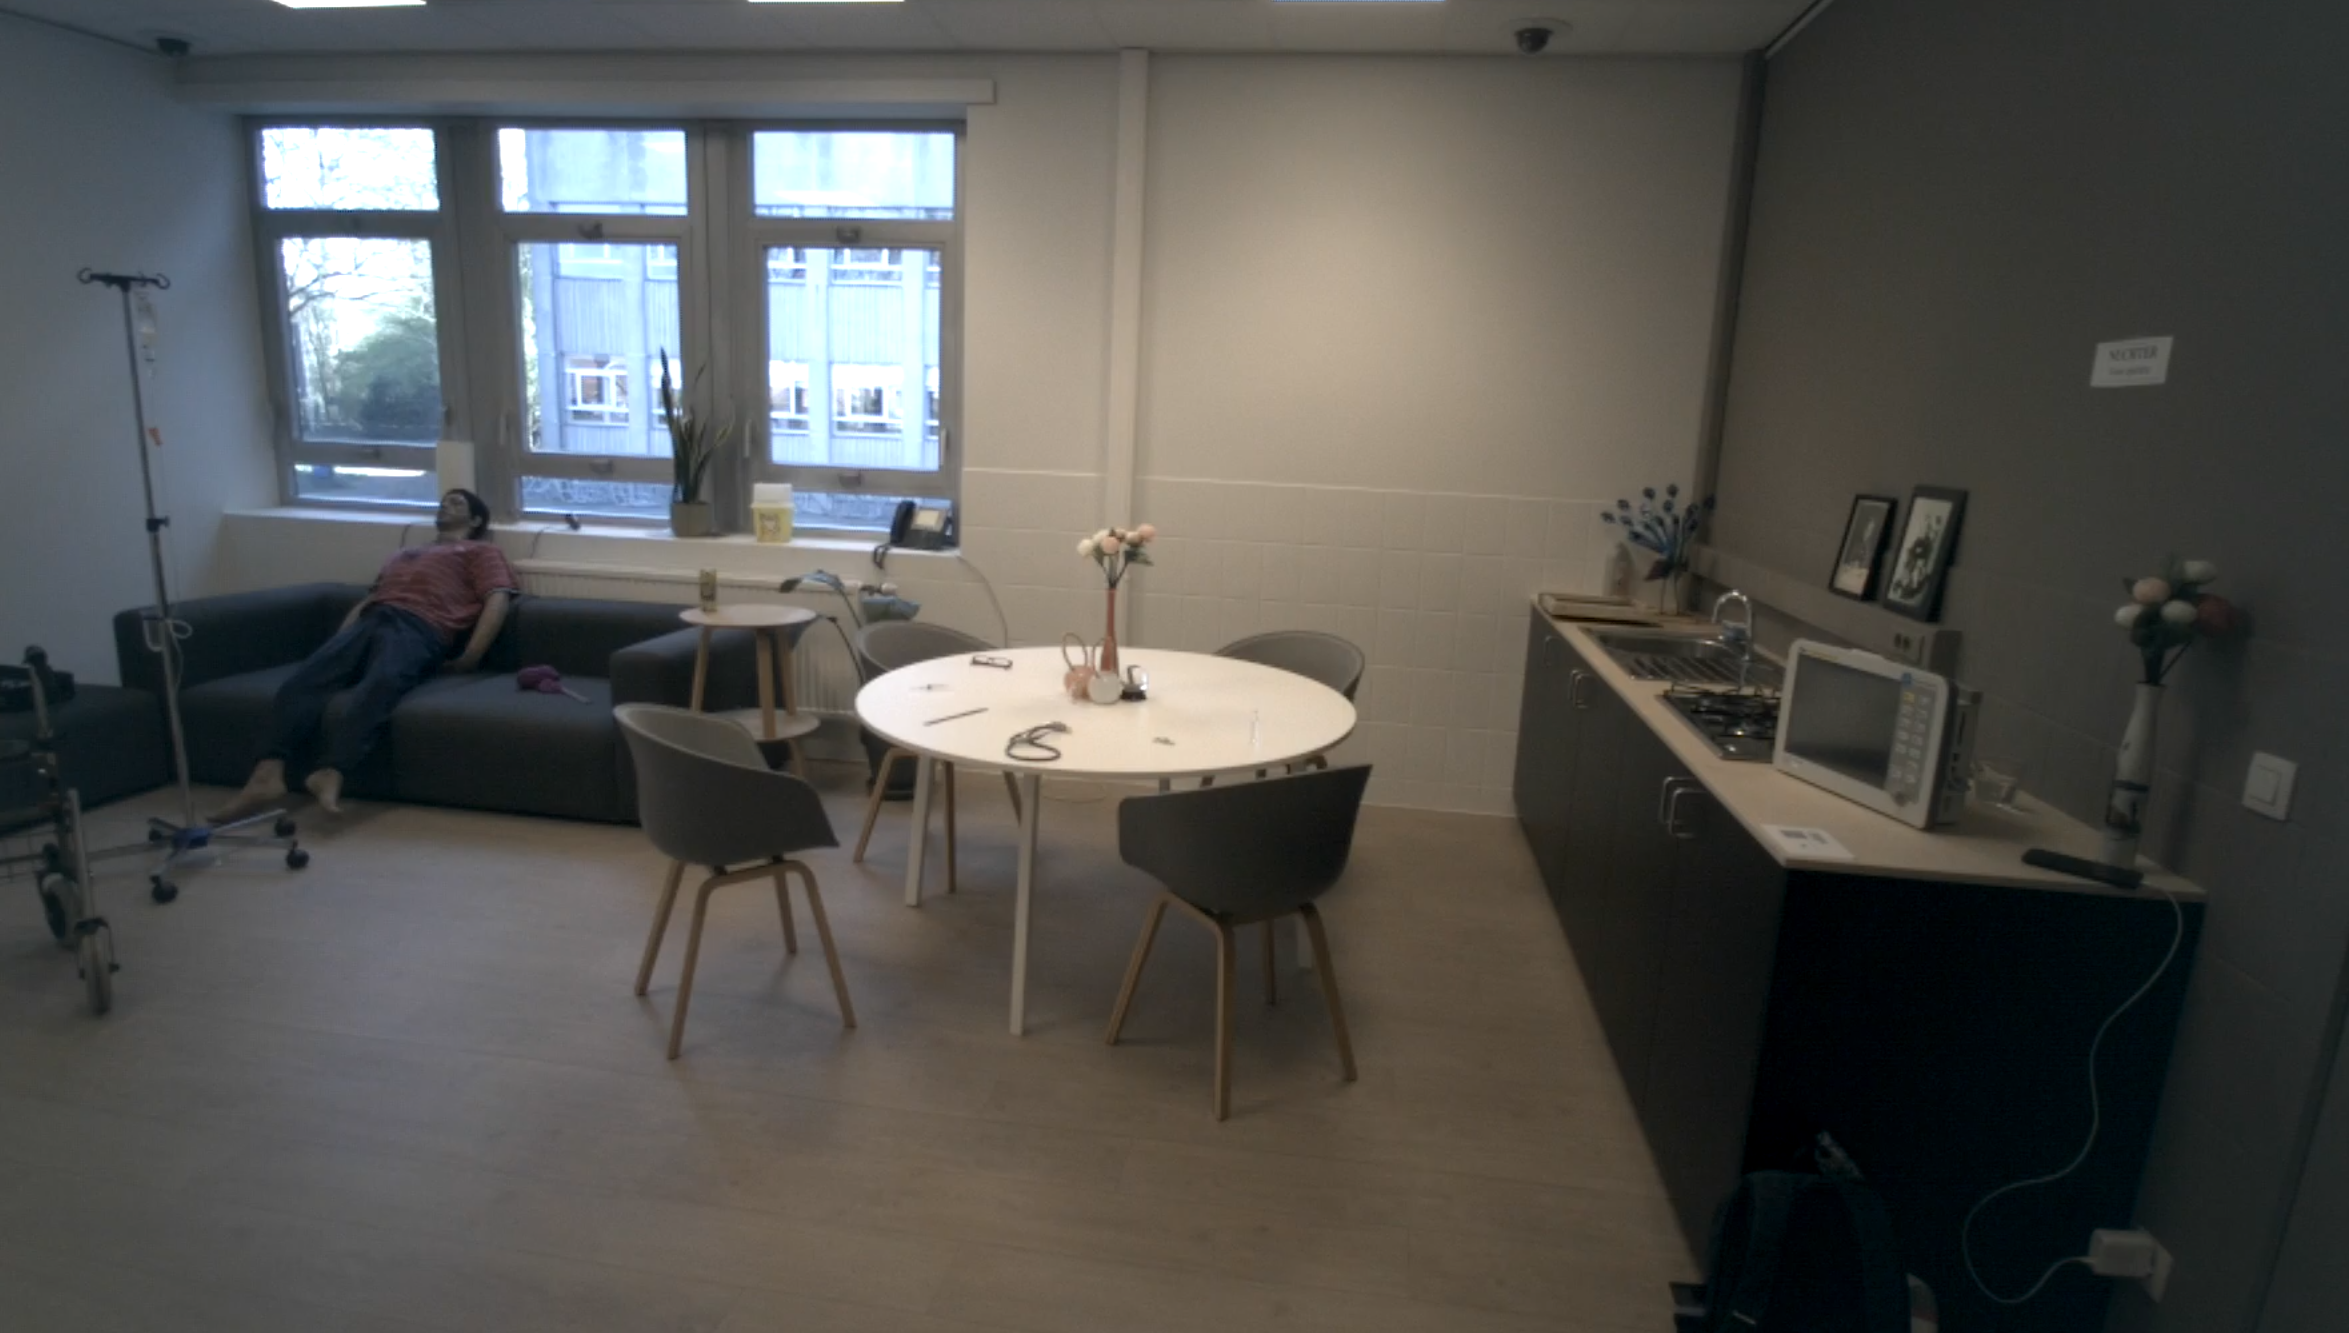
\includegraphics[width=1\textwidth]{zorglab.png}
  \caption[]{\label{fig:zorglab} De woonkameromgeving in het Zorglab van HoGent.}
\end{figure}

Het Zorglab beschikt over een uitgebreid assortiment aan objecten die ingezet kunnen worden tijdens simulatietrainingen. 
Uit deze collectie werden voor 15 specifieke objecten geselecteerd (zie Figuur~\ref{fig:object_grid}).
Dit aantal werd gekozen als een pragmatisch compromis tussen het verkrijgen van voldoende variatie in objecttypes 
die relevant zijn voor de zorgcontext en de technische uitdagingen, en het behouden van een haalbare werklast voor de latere annotatie van de grondwaarheid.
Deze objecten werden vervolgens in de woonkameromgeving geplaatst.

\begin{figure}[H]
  \centering
  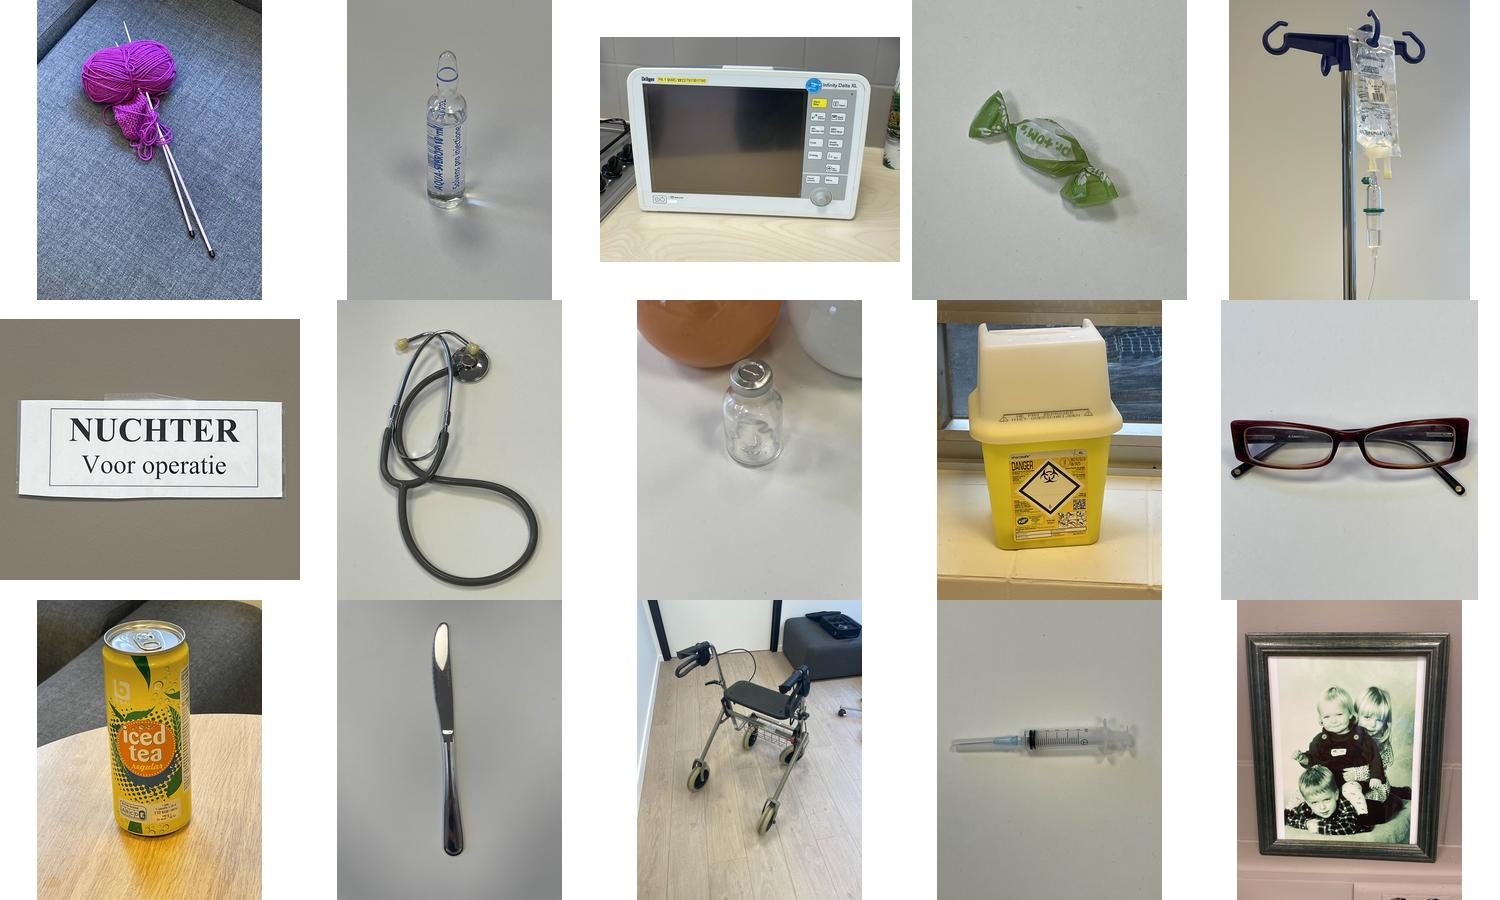
\includegraphics[width=0.8\textwidth]{object_grid.jpg}
  \caption[]{\label{fig:object_grid} De geselecteerde objecten voor het experiment. Van links naar rechts en van boven naar beneden: 
  een bol wol, een ampule met vloeistof, een monitor, een snoepje, een infuus, een indicator "Nuchter voor operatie", een stethoscoop, een transparante ampule, een naaldcontainer, een bril, een blikje iced tea, een keukenmes, een rollator, een spuit, een fotokder. 
  }
\end{figure}

Elk van deze objecten werd geselecteerd om redenen die zowel te maken hebben met de zorgcontext als met de technische haalbaarheid van de detectie:
\begin{itemize}
  \item \textbf{Bol wol}: Indicatief voor een hobby activiteit van de patiënt, en kan interessant zijn als gespreksonderwerp.
  \item \textbf{Ampule met vloeistof}: Een veelvoorkomend medisch object, hier specifiek gekozen voor de kleine afmetingen en de reflecterende eigenschappen van het glas.
  \item \textbf{Monitor}: Monitor waarop parameters (bv. bloeddruk/pols/ECG/...) aan de zorgverlener en/of patiënt worden getoond.
  \item \textbf{Snoepje}: Voornamelijk gekozen omwille van de kleine afmetingen met hoog kleurcontrast.
  \item \textbf{Infuus}: Het is belangrijk dat zorgverleners nakijken of een infuus voldoende is gevuld, en of het druppelmechanisme geactiveerd is.
  \item \textbf{Nuchter voor operatie}: Indicatoren zoals deze worden gebruikt in het zorglab om binnen een simulatie contextuele informatie te geven aan de studenten.
  \item \textbf{Stethoscoop}: Voornamelijk gekozen omwille van de complexe en potentieel variërende vorm van het object.
  \item \textbf{Transparante ampule}: Dit object is gekozen omwille van de reflecterende eigenschappen van het glas, en werd naast andere objecten geplaatst om de detectie potentieel te bemoeilijken.
  \item \textbf{Naaldcontainer}: Een naaldcontainer mag nooit binnen handbereik van een patiënt komen, en is dus een object dat zorgverleners altijd in het oog moeten houden.
  \item \textbf{Bril}: Een zorgverlener zou zich kunnen afvragen of een patiënt hun bril op heeft.
  \item \textbf{Blikje Iced Tea}: Bij een diabetespatiënt is het belangrijk dat de zorgverlener controleert of de patiënt geen ongezonde dranken consumeert.
  \item \textbf{Keukenmes}: Suicidepreventie is een belangrijk aandachtspunt in de zorg, en dit object kan potentieel gevaarlijk zijn voor patiënten met suïcidale gedachten. Hier werd een keukenmes gekozen, omdat het Zorglab geen gevaarlijke objecten ter beschikking had.
  \item \textbf{Rollator}: Dit object werd gekozen omwille van de grote afmetingen, en omdat een zorgverlener moet controleren of de rollator binnen bereik is van de patiënt.
  \item \textbf{Spuit}: Een veelvoorkomend medisch object, dat ook doorschijnend kan zijn maar toch een aantal specifieke visuele kenmerken heeft.
  \item \textbf{Fotokader}: Een fotokader kan eventueel familieleden of vrienden van de patiënt tonen, wat een gespreksonderwerp kan zijn.
\end{itemize}

\subsection{Deelnemers}

Voor het verzamelen van de evaluatieopnames werd een beroep gedaan op vrijwilligers. 
Deze werden gerekruteerd onder de studentenpopulatie op de campus van HoGent. 
Potentiële deelnemers werden voorafgaand aan hun deelname geïnformeerd over de doelstellingen en de aard van het onderzoek 
via een informed-consent formulier. Dit document bevatte tevens de voorwaarden voor deelname, 
waarbij benadrukt werd dat deelname volledig vrijwillig was en dat zij zich op elk gewenst moment zonder 
opgaaf van reden konden terugtrekken uit het experiment. 
Enkel na ondertekening van dit formulier werd de deelname bevestigd.

\subsection{Procedure}

\subsubsection{Proces bij Evaluatieopnames}

Om gestandaardiseerde data te verzamelen, werd een vaste procedure gevolgd voor elke opnamesessie met een deelnemer.

\begin{enumerate}
  \item \textbf{Voorbereiding object selectie:} Voorafgaand aan het experiment werden 15 unieke sets samengesteld, 
  elk bestaande uit vijf van de 15 geselecteerde objecten. 
  De keuze voor een beperkt aantal van vijf objecten per set werd gemaakt om meerdere redenen: 
  enerzijds om de benodigde tijd voor de latere annotatie van de ground-truth data per opname te beperken, 
  en anderzijds om de duur van elke individuele opnamesessie en daarmee de belasting voor de deelnemer te beperken.
  Elke set werd gevisualiseerd in een afzonderlijk PDF-document, met daarin duidelijke 
  afbeeldingen en de namen van de betreffende vijf objecten. 
  Bij het samenstellen van de sets werd gezorgd voor een evenwichtige spreiding, 
  zodat elk van de 15 objecten over het totaal van de sets ongeveer even vaak voorkwam.
  \item \textbf{Initiële briefing:} Bij aanvang van een opnamesessie werd aan de deelnemer eerst de specifieke 
  set van vijf objecten voor die sessie getoond aan de hand van het corresponderende PDF-document. 
  Tegelijkertijd wees de onderzoeker de fysieke locatie van elk van deze vijf objecten in de experimentele ruimte aan.
  \item \textbf{Uitleg procedure:} Na de identificatie van de objecten en hun locaties, 
  werd het volledige protocol van de observatietaak mondeling aan de deelnemer uitgelegd. 
  Dit omvatte de instructie om op een specifiek startpunt plaats te nemen, te wachten tot de onderzoeker een objectnaam noemt, 
  de blik op dat object te richten, er langzaam naartoe te lopen terwijl men blijft kijken, op signaal terug te keren naar het startpunt, 
  en dit proces te herhalen voor alle vijf objecten. 
  De deelnemer kreeg hierbij de gelegenheid om vragen te stellen, zodat de taakvereisten volledig duidelijk waren alvorens verder te gaan.
  \item \textbf{Setup eyetracker:} Vervolgens werd de Tobii Pro Glasses 3 eyetracker bij de deelnemer opgezet. 
  Hierna volgde een standaard kalibratieprocedure via de bijbehorende software. 
  De opname werd gestart na succesvolle kalibratie.
  \item \textbf{Start observatietaak:} De deelnemer werd verzocht plaats te nemen op het vooraf bepaalde startpunt in de ruimte. 
  De onderzoeker noemde vervolgens de naam van het eerste object uit de geselecteerde set.
  \item \textbf{Uitvoering observatietaak:} Bij het horen van de naam van een object, voerde de deelnemer de eerder uitgelegde instructie uit: 
  de blik op dat specifieke object richten en er vervolgens langzaam en rechtlijnig naartoe lopen, 
  terwijl de blik continu op het object gericht bleef. 
  Deze beweging naar het object toe was cruciaal om variatie in de kijkafstand te introduceren, 
  wat resulteert in opnames waarbij objecten van verschillende schijnbare groottes in het gezichtsveld van de camera verschijnen. 
  Op deze manier kunnen de effecten van kijkafstand op de detectieprestaties worden geëvalueerd.
  \item \textbf{Terugkeer en herhaling:} Na een signaal van de onderzoeker, keerde de deelnemer terug naar het oorspronkelijke startpunt. 
  Vervolgens noemde de onderzoeker het volgende object in de set, waarna stappen 6 en 7 werden herhaald.
  \item \textbf{Afronding sessie:} Nadat het vijfde object was bekeken en de deelnemer was teruggekeerd naar het startpunt, 
  werd de opname gestopt. De eyetracker werd afgenomen en de deelnemer werd bedankt voor hun medewerking.
\end{enumerate}

Het initiële streven was om ongeveer 15 evaluatieopnames te verzamelen, corresponderend met de 15 unieke objectsets. 
Dit aantal werd, net als het aantal geselecteerde objecten, als realistisch ingeschat met het oog op de benodigde tijd voor de 
latere handmatige annotatie van de ground-truth data. 
Uiteindelijk werd de beschreven procedure in totaal 14 maal herhaald met verschillende deelnemers, 
waarbij sommigen tweemaal deelnamen aan het experiment met een verschillende selectie van objecten. 
Door een administratieve fout tijdens de uitvoering werd echter één van de objectselecties dubbel opgenomen en een andere niet, 
waardoor de finale dataset evaluatieopnames bevat van 13 unieke objectselecties. 
Elke opname had een gemiddelde duur van ongeveer één minuut.

\subsubsection{Proces bij Kalibratieopnames}

Naast de evaluatieopnames werden, zoals eerder toegelicht, twee specifieke kalibratieopnames verricht door de onderzoeker.
De eerste kalibratieopname vond plaats met de 15 geselecteerde objecten in hun oorspronkelijke posities binnen de woonkameromgeving, 
identiek aan de setting voor de evaluatieopnames. 
Voor de tweede kalibratieopname werden dezelfde objecten vervolgens verplaatst naar een locatie met een significant afwijkende achtergrond. 
Het doel hiervan was specifiek om de invloed van de achtergrondcontext op de detectieprestaties van de modellen te kunnen beoordelen.
Aangezien beide opnames binnen een korte tijdsspanne werden gemaakt, bleven de lichtomstandigheden consistent tussen de twee kalibratieopnames.

% TODO: hier nog iets toevoegen?